\subsection{Anwendungsfälle von Cloud Computing}

\begin{figure}[h]
    \centering
    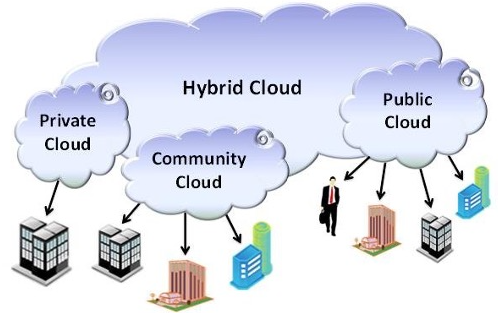
\includegraphics[scale=1]{sections/cloud-computing/images/cc-use-cases.png}
    \caption{Anwendungsfälle}
\end{figure}

\subsubsection{Private Cloud}

Dieses Bereitstellungsmodell wird vor allem in Unternehmen verwendet, das heißt diese Dienste sind nicht für die Öffentlichkeit zugänglich. Sie werden nur Unternehmensintern verwendet. Die Nutzer können standortunabhängig von diesen Cloud Computing Diensten Gebrauch machen, müssen aber Teil der gleichen Organisation sein. Die private Cloud ist die sicherste der Bereitstellungsmethoden. Der Grund dafür ist, dass Prozesse innerhalb des Unternehmens kontrolliert und verwaltet werden, ohne jegliche Leistungs- Sicherheitsbeschränkungen, die Dienste in der Public Cloud vielleicht benötigen. In der privaten Cloud ist es möglich, dass die fundamentale Infrastruktur der Cloud vom Unternehmen selbst, von Drittanbietern oder auch von Beiden verwaltet wird. Generell wird die Private Cloud in zwei unterschiedliche Arten unterteilt:

\begin{itemize}
    \item On-Premise Private Cloud
    \begin{sloppypar}
        Diese Art wird auch interne Cloud genannt. Sie bietet zusätzliche Sicherheit, dennoch kann sie in Größe und Skalierbarkeit stark eingeschränkt sein, da man selbst das Kapital für Hard- und Software, sowie Wartung und Instandhaltung aufbringen muss. Die interne Cloud eignet sich somit für Anwendungen, die die volle Kontrolle sämtlicher Ressourcen verlangen.
    \end{sloppypar}
    \item extern gehostete Private Cloud
    \begin{sloppypar} 
        Hier wird das Hosten der Cloud von einem Drittanbieter übernommen. Diese Anbieter fördern eine restriktive Cloud Computing-Umgebung mit vollständiger Vertraulichkeit. Diese Art der Private Cloud wird für Institutionen empfohlen, die das Kapital für eine interne Private Cloud nicht aufbringen können.
    \end{sloppypar} 
\end{itemize}

\subsubsection{Public Cloud}

Eine Public Cloud ist für die Öffentlichkeit zugänglich und kann von einem Unternehmen, einer staatlichen Einrichtung oder Organisation verwendet werden. Die Cloud ist jedoch im Besitz eines Drittanbieters. Hierbei greift der Nutzer über Schnittstellen auf die CC-Dienste des Cloud-Besitzers zu.

\subsubsection{Community Cloud}

In der Community Cloud wird die Infrastruktur einer Cloud von mehreren Unternehmen oder Institutionen mit ähnlichen oder gemeinsamen Zielen verwendet. Die Infrastruktur kann entweder von einer Organisation oder mehreren Organisationen verwaltet werden.

\subsubsection{Hybrid-Cloud}

Diese Variante ist eine Kombination aus einer oder mehreren privaten und öffentlichen Cloud, die aber als getrennte Einheiten fungieren. Diese Einheiten werden durch eine Protokollen und Standardisierungen verbunden. Dieses Modell wird hauptsächlich verwendet, wenn man die Vorteile der unterschiedlichen CC-Bereitstellungsoptionen kombinieren möchte. Beispielsweise, ein Unternehmen möchte die Datenspeicherung auf einer privaten Cloud realisieren, und andere Aufgaben mithilfe einer öffentlichen Cloud erledigen.

\subsubsection{Azure Cloud}

Microsoft Azure ist ein Cloud-Computing-Dienst von Microsoft. Azure bietet eine Reihe von Software as a Service (SaaS), Plattform as a Service (PaaS) und Infrastruktur as a Service (IaaS) Optionen, für die Bereitstellung von Anwendungen und Diensten, auf einer von Microsoft verwalteten Rechenzentrumsinfrastruktur an. Mit 50 Betriebsregionen bietet Azure mehr als jeder andere Cloud-Anbieter.

